\documentclass[12pt]{report}

\usepackage[francais]{babel}

\usepackage[utf8]{inputenc}

\usepackage[a4paper,left=2cm,right=2cm,top=2cm,bottom=2cm]{geometry}
\usepackage[pdftex]{graphicx}
\usepackage{float}

\setlength{\parindent}{0.8cm}
\setlength{\parskip}{1ex plus 0.5ex minus 0.2ex}
\newcommand{\hsp}{\hspace{20pt}}
\newcommand{\HRule}{\rule{\linewidth}{0.5mm}}


\date{April 2017}

\begin{document}
	\begin{titlepage}
		
		\begin{center}
			

			
\includegraphics[scale=0.11]{logo-um.png}~\\[1.5cm]
			
			\textsc{\LARGE Faculté des Sciences de Montpellier}\\[2cm]
				
			\textsc{\Large Rapport de projet - Licence 2ème année}\\[0.5cm]
			\textsc{\Large Informatique - TER (HLIN405)}\\[0.5cm]
			\textsc{\Large 2016-2017}\\[1.5cm]
				
			\HRule \\[0.4cm]
			{ \huge \bfseries Jeu de cartes en ligne\\[0.4cm] }
			
			\HRule \\[2cm]
				
			\begin{flushleft}
				\large	Maëlle \textsc{Beuret}\\[0.5cm]
				\large	Bachar \textsc{Rima}\\[0.5cm]
				\large	Othmane \textsc{Farajallah}\\[0.5cm]
				Début du projet : 18 janvier 2017		
			\end{flushleft}
			
			\vfill
				
			
\includegraphics[scale=0.3]{logo-fds.jpg}~	
				
		\end{center}
	\end{titlepage}
	
\tableofcontents

\chapter*{Introduction}
\addcontentsline{toc}{chapter}{Introduction}
    
    \section*{Présentation du jeu}
    \addcontentsline{toc}{section}{Présentation du jeu}
    
    Les Voyageurs de Kaeraly est un jeu de cartes coopératif en ligne. Le but des joueurs est de tuer le Loup Alpha. Pour cela, il leur faudra traverser différentes zones (forêt, rivière, plaine) à l'aide d'objets trouvés aléatoirement lors de leur voyage, équiper de l'armure ou des armes, et utiliser des potions afin d'améliorer leurs statistiques d'attaque et de défense. 
    
    
    Inspiré des jeux de rôle sur table ainsi que des jeux de société tels que le Munchkin, nous avons eu l'idée de créer ce jeu en collaboration avec des illustrateurs venant de Suisse, de Roumanie et des Pays Bas, afin de partager l'expérience d'un jeu de société à distance, tout en ayant l'opportunité de s'améliorer dans nos domaines respectifs (graphisme et développement informatique). Ce projet faisant appel à de nombreuses technologies informatiques, nous avons décidé d'en faire notre projet universitaire de deuxième année de licence.
    
    \section*{Cahier des charges}
    \addcontentsline{toc}{section}{Cahier des charges}
    
    Afin de réaliser ce projet, nous devions utiliser le langage JavaScript (langage de programmation Web), avec notamment la bibliothèque D3 pour le graphisme, ainsi que Node.js (plateforme logicielle et événementielle légère en JavaScript, permettant de mettre des réseaux en place) et les WebSockets (technologie permettant la communication interactive entre un navigateur (client) et un serveur) pour l'architecture client-serveur. 
    
    
    Il nous fallait également mettre en place un système de tour par tour afin que les joueurs ne puissent interagir avec les cartes que lorsque leur tour est activé. Le jeu étant multijoueurs, il nous fallait également intégrer le passage automatique du tour si un joueur s'absente pendant trop longtemps. 
    
    
    Afin de rendre le jeu le plus dynamique et ergonomique possible, nous devions mettre en place l'interaction avec les cartes optimale : pouvoir cliquer directement sur la pile pour tirer une carte, pouvoir sélectionner dans la main la carte que l'on souhaite utiliser, etc. 
    
    Enfin, nous avions besoin de créer et gérer une base de données afin de stocker toutes les cartes du jeu.
    
\chapter{Organisation du projet}

    \section{Organisation du travail}
    
    \section{Choix des outils de développement}
    
\chapter{Conception}

	Avant de commencer la phase de programmation, nous avons modélisé nos objets et préparé une maquette visuelle de notre programme. Nous avons également choisi les technologies nécessaires et pertinentes pour notre projet. 
    
    \section{Modélisation des objets}
    
    \section{Maquette graphique}
    
    Afin de visualiser le rendu de notre jeu et avoir une référence lors du code de l'affichage, nous avons réalisé une maquette graphique de notre programme (voir figure \ref{fig:maquette}). Les illustrations n'étant pas encore réalisées à cette étape, nous avons utilisé d'autres dessins d'une artiste collaborant avec nous. Le but de cette maquette n'étant pas de définir l'aspect final mais l'emplacement des objets, elle est minimaliste et le rendu final du jeu devait être plus esthétique.\\[1.5cm]
    
    \begin{figure}[h!]
    	\centering
	    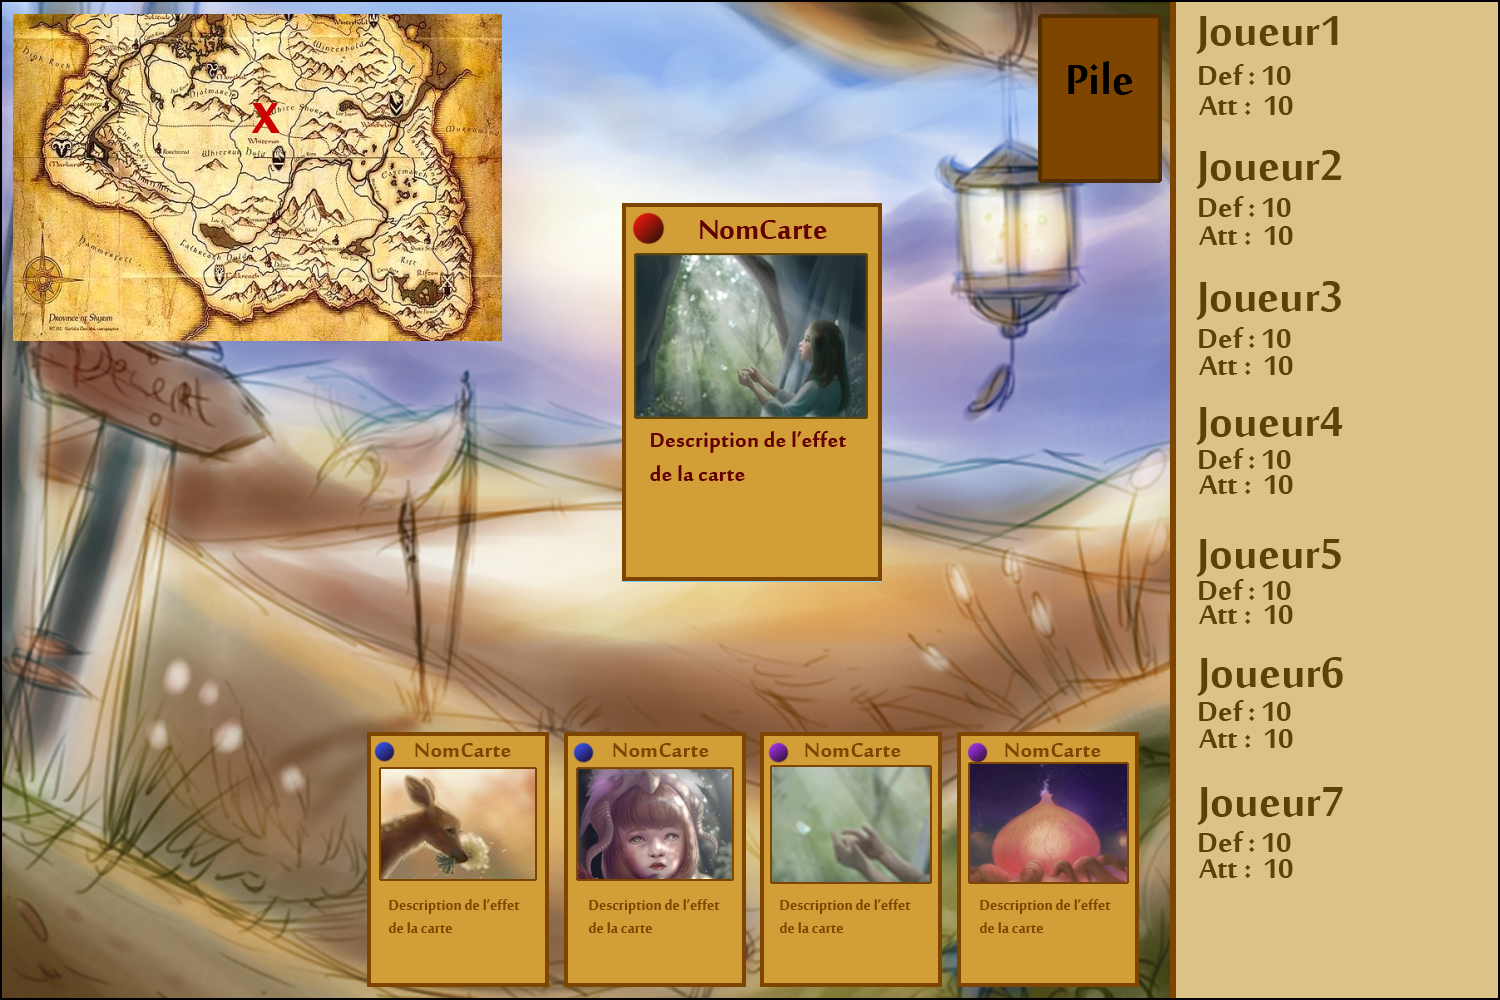
\includegraphics[scale=2.8]{mock-up.png}
	    \caption{Maquette graphique du jeu.}
	    \label{fig:maquette}
    \end{figure}

    
    \section{Architecture du site}
    
    \section{Choix des technologies}
    
    \section{Base de données}
    
\chapter{Développement}
    
    \section{Gestion de l'événementiel}
    
    \section{Graphismes}
        
        \subsection{Réalisation des images}
        
        Afin d'obtenir un rendu esthétique pour le jeu, nous avons créé des illustrations avec l'aide des illustrateurs avec lesquels nous avons collaboré. Ceux-ci se sont chargés de faire les fonds pour les environnements plaine et rivière, ainsi que les deux épées présentes sur les cartes du jeu. 
        
        \begin{figure}[h!]
	       	\centering
           	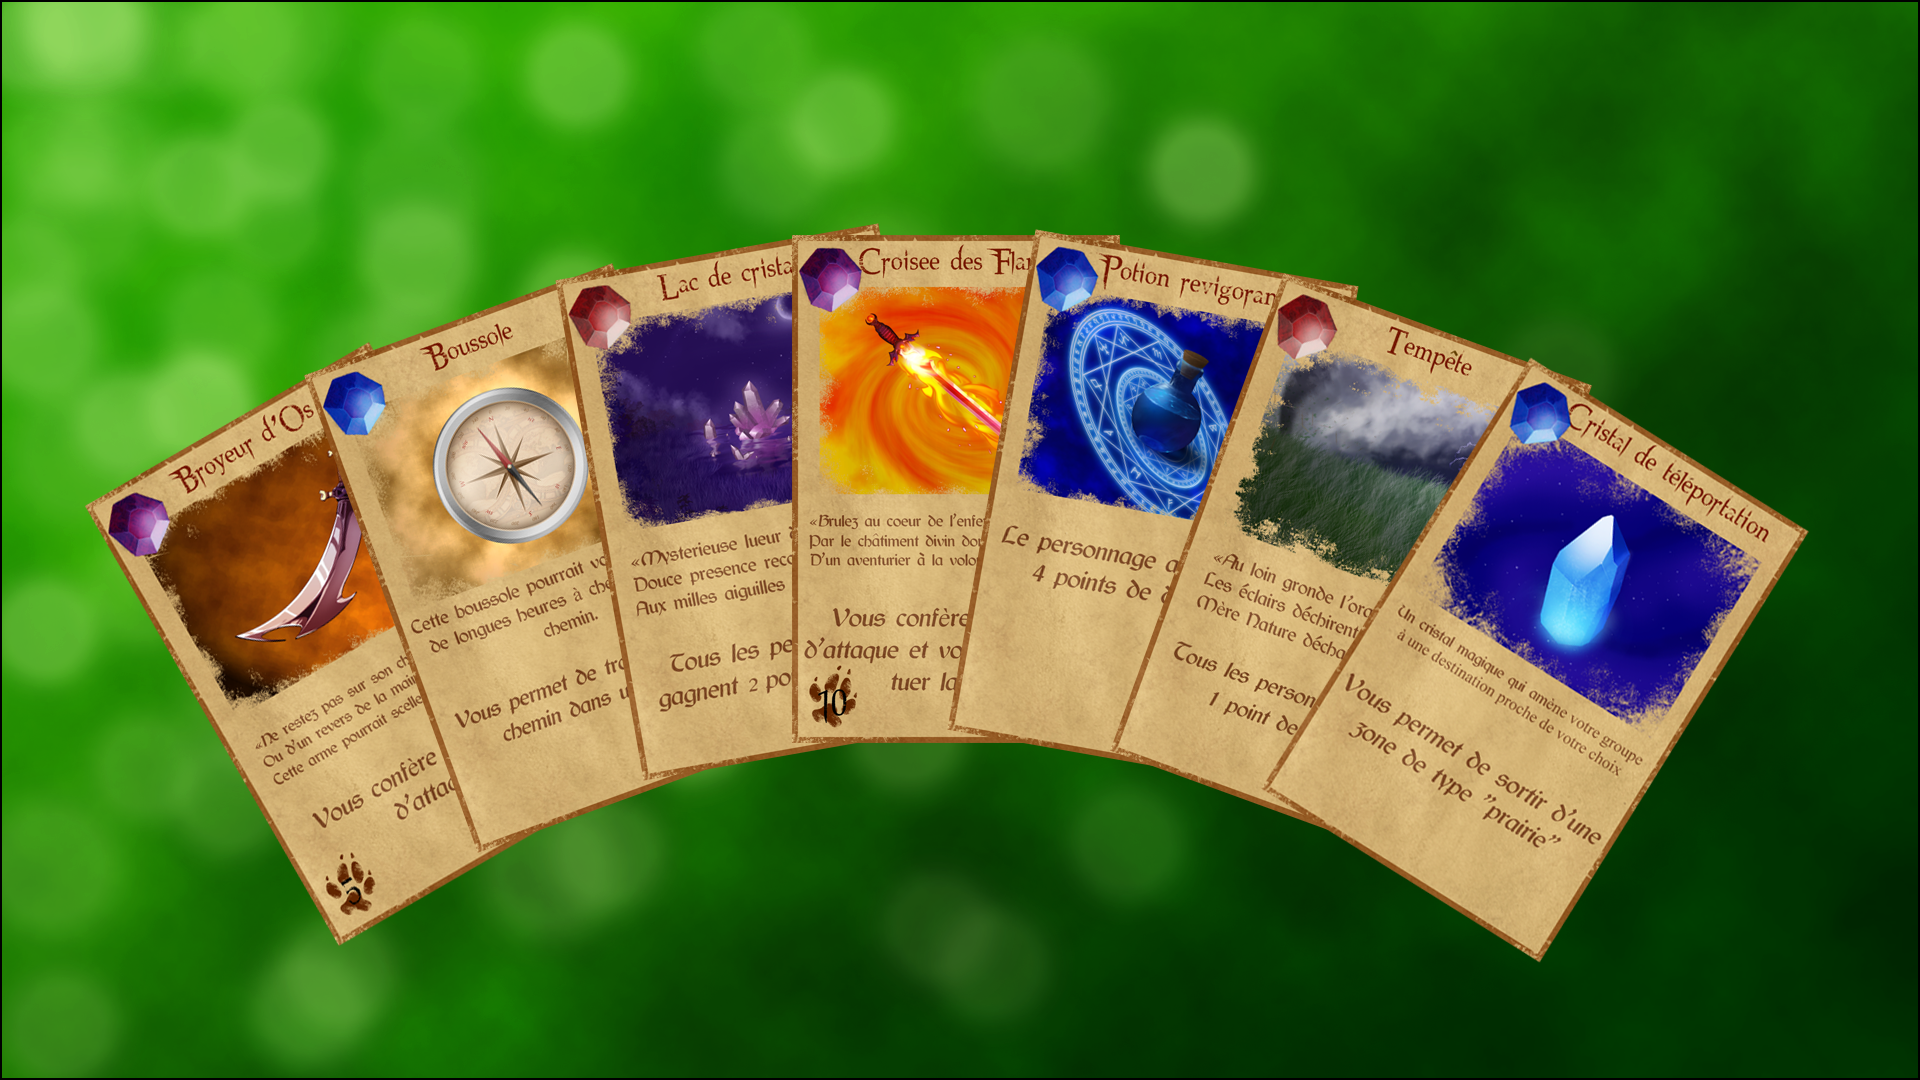
\includegraphics[scale=0.4]{cards.png}
           	\caption{Exemple de cartes crées ainsi que le fond du site.}
           	\label{fig:cartes}
        \end{figure}
        
        Nous nous sommes chargés de réaliser, à l'aide d'un logiciel de dessin assisté, les autres illustrations pour les cartes, les éléments de décoration des cartes (gemme indiquant le type, symboles d'attaque et de défense, effets visuels. Voir figure \ref{fig:cartes}), le fond pour l'environnement "forêt", le dos de carte pour la pile, ainsi que les autres éléments décoratifs du site (texture de bois, fond).
        
        Chaque illustration nous a demandé plusieurs heures de travail, et il était prévu que nos collaborateurs réalisent la majeure partie des graphismes. Cependant, par manque de temps de leur part, nous avons dû investir plus de temps que prévu dans cette partie du projet. 
        
        
        \subsection{Affichage graphique en JavaScript}
        
        Pour afficher les différents éléments du jeu (cartes de jeu, pile, carte de la zone) nous avons utilisé la bibliothèque D3. Celle-ci permet de manipuler des éléments SVG (Scalable Vector Graphics, format d'images vectorielles). 
        
        Nous avons créé une zone SVG recouvrant toute la partie du site dédiée au jeu, de la manière suivante :
        
        \begin{verbatim}
        var svg = d3.select('#svgWin')
                    .append('svg')
                    .attr('width', 900)
                    .attr('height', 650);
        \end{verbatim}
        
        Ici, 'svgWin' désigne la balise html <div> ayant pour attribut "id = 'svgWin' ". La fonction append('svg') permet de créer un élément SVG fils de "svgWin". Nous lui attribuons ensuite une largeur et une hauteur correspondant à la taille de la zone dédiée au jeu. Nous avons procédé de la même manière pour les images, avec des objets de type "svg:image", en y ajoutant les attributs "x" et "y" pour la position dans la zone SVG. 
        
        Outre l'affichage d'image, nous avons également affiché la carte des zones du jeu à l'aide de D3. Pour cela, nous avons créé des hexagones que nous avons rempli de couleurs correspondant à l'environnement de la zone représentée par chaque hexagone. Le dessin des hexagones est réalisé à l'aide de "path", qui permet de dessiner les contours d'une forme (rectangle, cercle, simple ligne...).
        
        Nous avons également utilisé D3 pour effectuer un zoom sur les cartes en main lors du passage de la souris sur celles-ci afin que les joueurs puissent lire les effets de leurs cartes plus facilement. 
        
    
\chapter{Manuel d'utilisation}

    \section{Navigation sur le site}
    
    Le site comporte 3 différentes pages, accessibles depuis la barre de menu en haut. La page principale est celle concernant uniquement le jeu, avec en haut à gauche le champ de texte pour entrer un pseudo et se connecter, ainsi que le bouton permettant de quitter la partie. Au centre de la page se trouve la fenêtre de jeu.
    
    Il est possible de consulter les règles du jeu en cliquant sur le lien "Règles" dans le menu. On y trouve toutes les informations nécessaires pour une partie.
    
    Enfin, tous les contributeurs du projet (les artistes ayant collaboré avec nous ainsi que nous-mêmes) sont listés sur la page "crédits", également accessible à l'aide du lien du même nom dans le menu. 
    
    \section{Fonctionnement du jeu}
    
    Une fois la partie commencée, chaque joueur joue tour à tour. Un tour consiste à tirer une carte de la pile, en cliquant sur l'image du dos de carte sur la gauche de la fenêtre de jeu. Le joueur peut alors décider de prendre la carte ou la jeter, en cliquant sur le bouton correspondant qui s'affichera en même temps que la carte tirée. 
    
    Les cartes que le joueur décide de prendre s'affichent en bas de la fenêtre de jeu. La main du joueur est limitée à cinq cartes, par conséquent, si l'on a déjà une main pleine on ne peut pas prendre de nouvelle carte sans se débarrasser d'une autre. Différentes interactions sont possibles avec les cartes que l'on a en main : en cliquant sur une carte, des choix s'offrent à nous, modélisés par des boutons. S'il s'agit d'une carte équipable, on peut l'équiper. S'il s'agit d'une carte utilisable (potion ou objet permettant de changer de lieu), on peut l'utiliser. Dans tous les cas, il est possible de jeter la carte si on décide qu'elle ne nous est plus d'aucune utilité ou que l'on souhaite faire de la place dans notre main. 
    
    Dans le cas de l'utilisation d'un objet permettant de changer de zone, il faut choisir la zone suivante dans laquelle les joueurs veulent se placer. Il est impossible de reculer, seules trois directions sont possibles : haut, droite, bas. 
    
    Un joueur dispose d'un temps imparti pour terminer son tour. Il est possible de passer son tour après avoir réalisé toutes les actions que l'on souhaitait faire en cliquant sur le bouton "Terminer le tour". Si le joueur ne clique pas sur ce bouton dans les temps, le tour passe automatiquement au joueur suivant afin d'éviter que la partie ne soit bloquée par un joueur inactif. 
    
\chapter*{Conclusion}
\addcontentsline{toc}{chapter}{Conclusion}

    \section*{Bilan}
    \addcontentsline{toc}{section}{Bilan}
    
    \section*{Perspectives}
    \addcontentsline{toc}{section}{Perspectives}

    \section*{Apports personnels du projet}
    \addcontentsline{toc}{section}{Apports personnels du projet}

\end{document}
